\documentclass[aspectratio=169,11pt]{beamer}
\usetheme{default}
\usefonttheme{professionalfonts}
\renewcommand{\familydefault}{\sfdefault}
\setbeamertemplate{navigation symbols}{}
\setbeamertemplate{footline}[frame number]
\setbeamertemplate{itemize items}[circle]
\usepackage[T1]{fontenc}
\usepackage{graphicx}
\usepackage{booktabs}
\usepackage{tabularray}
\UseTblrLibrary{booktabs}
\usepackage{xcolor}
\usepackage[numbers]{natbib}
\graphicspath{{../../output/figures/}}

\title{Digital Payments (UPI) and Financial Inclusion across Indian States}
\subtitle{B.Tech Project, Part I}
\author{Devansh Gupta}
\institute{Supervisor: Prof. Rudra Prakash Pradhan (VGSOM)\\IIT Kharagpur}
\date{November 2026}

\begin{document}

% ---- 1. Title
% Notes: I present Part I of my B.Tech project. The topic is UPI adoption and financial inclusion across Indian states. Prof. Pradhan supervises the project.
\begin{frame}[plain]
\titlepage
\end{frame}

% ---- 2. Motivation
% Source: proposal.txt (Background, Problem statement)
% Notes: UPI started in 2016 and NPCI operates it. The Jan Dhan drive started in 2014. Policy discussion assumes that digital payments widen access to finance. The state-level evidence is thin. We do not know if adoption leads to inclusion, or if more inclusive states adopted faster.
\begin{frame}{Motivation}
\begin{itemize}
\item UPI was launched in 2016 and is operated by NPCI. % proposal.txt
\item The Jan Dhan account drive began in 2014. % proposal.txt
\item Policy discussion assumes that digital payments widen access to formal finance and support growth. % proposal.txt
\item The evidence at state level is thin. % proposal.txt
\item It is unclear whether higher adoption leads to deeper financial inclusion, or whether states that were already more inclusive adopted faster. % proposal.txt
\end{itemize}
\end{frame}

% ---- 3. RQs and hypotheses
% Source: proposal.txt (Research questions and hypotheses)
% Notes: These are the four research questions and their hypotheses from my proposal. BTP-I does not estimate them. BTP-II does.
\begin{frame}{Research questions and hypotheses}
\begin{itemize}
\item RQ1: Does higher digital payment adoption raise financial inclusion in a state? (H1: yes, positively.)
\item RQ2: Does adoption contribute to state-level economic growth after controlling for other drivers? (H2: yes, positively.)
\item RQ3: Is the causality bidirectional? (H3: yes; inclusion also encourages adoption.)
\item RQ4: Does the effect differ between better-connected and weaker-infrastructure states? (H4: stronger where internet access is higher.)
\end{itemize}
\end{frame}

% ---- 4. Literature and gap
% Source: thesis/btp1/chapters/ch2_literature.tex; proposal.txt; spec Key references
% Notes: The review has four parts: finance and growth, FI and ICT in Indian states, digital payments and UPI, and the methods used. The gap: no peer-reviewed state-panel study of UPI adoption, FI and growth with a causality test.
\begin{frame}{Literature and gap}
\begin{itemize}
\item Finance and economic growth.
\item Financial inclusion and ICT in Indian states \citep{pradhan2021tfsc,pradhan2021ael}.
\item Digital payments and UPI \citep{reddy2024icrier}.
\item Methods: panel Granger causality \citep{dumitrescu2012}; panel VAR \citep{love2006,abrigo2016}.
\item \textbf{Gap:} no peer-reviewed state-panel study of UPI adoption, financial inclusion and growth with a causality test.
\end{itemize}
\end{frame}

% ---- 5. Data availability
% Source: thesis/progress/part1.tex (Data findings so far); spec Section 1
% Notes: These are the data findings. NPCI state data starts in April 2025. The RBI index is national only. PMJDY has one snapshot only.
\begin{frame}{Data availability}
\begin{itemize}
\item NPCI publishes state-wise UPI data only from April 2025 \citep{npci_upi_state,medianama2025npci}. % part1.tex
\item One analysis reports that 27.5\% of FY25 UPI volume has no state attribution \citep{dataful2026upi}. % part1.tex
\item The RBI Financial Inclusion Index is published for India only, not for states \citep{rbi_fiindex2025}. % part1.tex
\item The PMJDY state-wise statistics are one snapshot (21 October 2026) with no history \citep{pmjdy_statewise}. % part1.tex
\end{itemize}
\end{frame}

% ---- 6. PhonePe Pulse as proxy
% Source: thesis/progress/part1.tex (ingestion, totals table); spec Section 1
% Notes: PhonePe Pulse is the adoption proxy because it has state-level quarterly data from 2018Q1. Total transactions rose from 139.98 million in 2018Q1 to 38664.29 million in 2026Q2. The proxy needs supervisor approval (Task 0 open item).
\begin{frame}{PhonePe Pulse as proxy}
\begin{itemize}
\item PhonePe Pulse commit \texttt{257bf38} \citep{phonepe_pulse}. % part1.tex
\item Coverage: 2018Q1 to 2026Q2, 35 state ids. % part1.tex
\item Three variables: transaction count, amount (Rs.), registered users. % part1.tex
% Command: PYTHONPATH=src/py .venv/bin/python -c "import pandas as pd; from btpdata import npci; p=pd.read_csv('data/final/panel_quarterly.csv'); m=npci._load(npci.RAW)
%   for q,ms in [('2025Q2',['2025-Apr','2025-May','2025-Jun']),('2026Q2',['2026-Apr','2026-May','2026-Jun'])]: v=sum(npci._number(r['volume_in_mn']) for k in ms for r in npci._state_rows(m[k]))*1e6; c=p[p.period==q].phonepe_count.sum(); print(q,c,v,round(c/v,3))"
%   (output: 2025Q2 31134210599 54965890000 0.566; 2026Q2 38664285691 68588630000 0.564)
%   NPCI volume: all rows without a district, unclassified row included.
\item PhonePe Pulse transaction count / NPCI UPI volume (all rows, unclassified included): 0.566 (2025Q2), 0.564 (2026Q2).
\item Total transactions: 139.98 million in 2018Q1; 38,664.29 million in 2026Q2. % part1.tex Table
\item Supervisor approval of the proxy is an open item. % part1.tex, part2.tex
\end{itemize}
\end{frame}

% ---- 7. Variables and sample
% Source: output/tables/summary_stats.tex; thesis/progress/part2.tex (Panel); spec Section 3
% Notes: The main sample has 30 ids: 28 states, Delhi, and Jammu and Kashmir with Ladakh. The quarterly panel has 1190 rows. The table gives summary statistics for the main sample: 1,020 observations.
\begin{frame}{Variables and sample}
\begin{itemize}
\item Main sample: 30 ids (28 states, Delhi, Jammu and Kashmir including Ladakh). % part1.tex
\item Panel: 1190 rows, 35 state ids, 34 quarters (2018Q1 to 2026Q2). % part2.tex
\item Money values are real (state CPI, base 2012 = 100). % part2.tex
\end{itemize}
\vspace{0.5em}
\begin{center}
\footnotesize
\resizebox{0.95\textwidth}{!}{\begin{tabular}{lrrrrr}
\toprule
Variable & N & Mean & SD & Min & Max \\
\midrule
Transactions per person (count) & 1,020 & 8.35 & 13.00 & 0.02 & 100.30 \\
Real value per person (Rs., 2012 prices) & 1,020 & 6,130.33 & 8,603.22 & 17.48 & 62,328.19 \\
Registered users per 1,000 & 1,020 & 274.04 & 193.56 & 6.99 & 943.50 \\
Population (millions) & 1,020 & 45.66 & 50.37 & 0.66 & 243.31 \\
CPI & 1,020 & 169.87 & 21.69 & 131.37 & 226.23 \\
\bottomrule
\end{tabular}
}
\end{center}
\end{frame}

% ---- 8. Method plan
% Source: spec Section 4 (Econometric sequence) and Section 5
% Notes: Step 0 is done in BTP-I. Steps 1 to 3 are in BTP-II. Results are reported as predictive (Granger) causality, not as causal effects.
\begin{frame}{Method plan}
\begin{itemize}
\item Step 0: description and validation (trends, maps, $\sigma$- and $\beta$-convergence, PhonePe against NPCI). % spec
\item Step 1: series properties (Pesaran CD test, CIPS or IPS, Pedroni cointegration). % spec
\item RQ1 and RQ4: fixed and random effects, Hausman test, Driscoll--Kraay standard errors. % spec
\item RQ3: Dumitrescu--Hurlin test; panel VAR by GMM. % spec
\item RQ2: annual tier, fixed effects and system GMM. % spec
\item Results are reported as predictive (Granger) causality, not as causal effects. % spec
\end{itemize}
\end{frame}

% ---- 9. Adoption trend
% Source: thesis/btp1/chapters/ch5_results.tex (caption of fig:trend)
% Notes: The figure shows the median and interquartile range across states of the natural log of real value per person per quarter, 2018Q1 to 2026Q2, main sample.
\begin{frame}{Adoption trend}
\centering
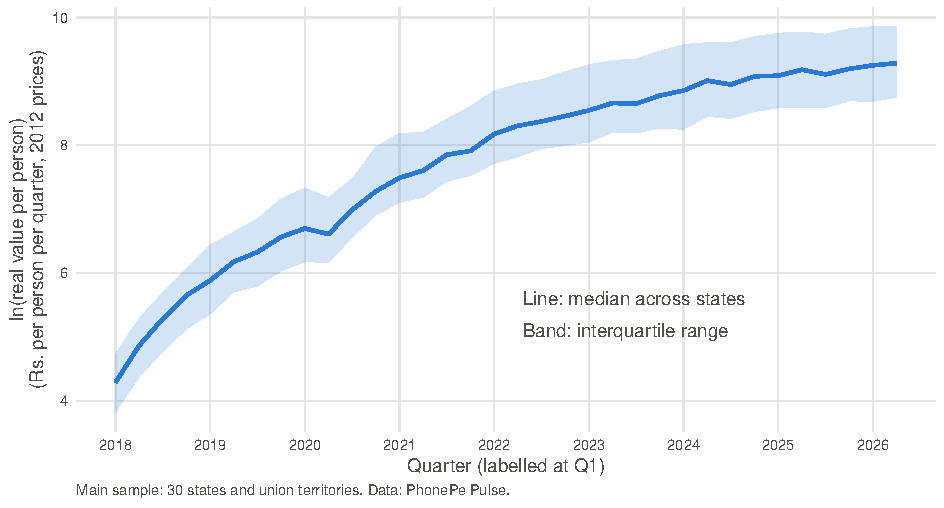
\includegraphics[height=0.74\textheight,keepaspectratio]{adoption_trend_main.pdf}

\vspace{0.3em}
{\footnotesize Median and interquartile range across states of ln real value per person per quarter (Rs., 2012 prices), 2018Q1--2026Q2, main sample. Data: PhonePe Pulse; MoSPI state CPI; NCP 2020.\par}
\end{frame}

% ---- 10. Maps
% Source: thesis/btp1/chapters/ch5_results.tex (caption of fig:maps)
% Notes: Both maps show real value per person per quarter with the same log colour scale. The left map is 2018Q4. The right map is 2026Q2.
\begin{frame}{Maps: 2018Q4 and 2026Q2}
\centering
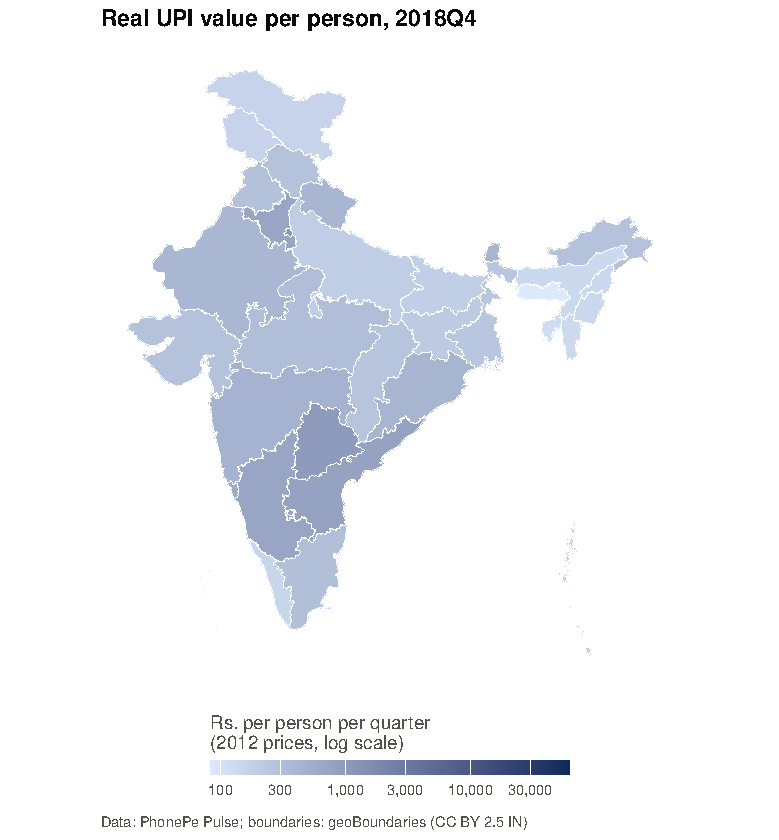
\includegraphics[width=0.48\textwidth,height=0.74\textheight,keepaspectratio]{adoption_map_2018Q4.pdf}\hfill
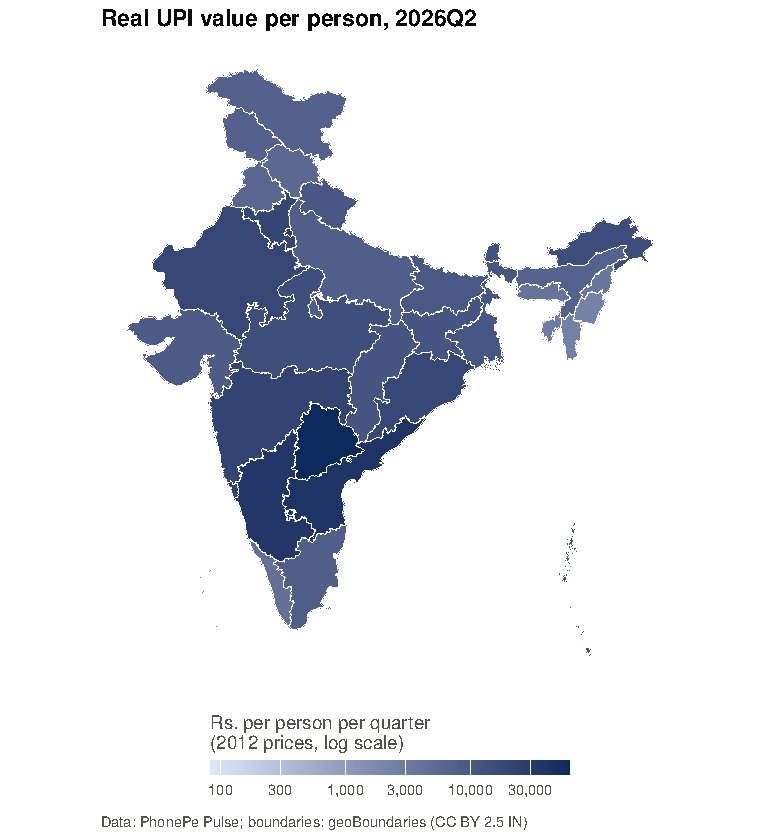
\includegraphics[width=0.48\textwidth,height=0.74\textheight,keepaspectratio]{adoption_map_2026Q2.pdf}

\vspace{0.3em}
{\footnotesize Real value per person per quarter (Rs., 2012 prices); log colour scale, same scale in both panels. Left: 2018Q4. Right: 2026Q2.\par}
\end{frame}

% ---- 11. Convergence
% Source: output/figures/sigma_convergence.pdf; output/tables/beta_convergence.tex
% Notes: Left: sigma-convergence, the coefficient of variation across states over time. Right: beta-convergence, N = 30. The slope on ln(initial level) is 0.0177 (0.0138) for real value per person and -0.0030 (0.0128) for transactions per person. R-squared is 0.056 and 0.002. (Values from output/tables/beta_convergence.tex after the December 2025 CPI link.)
\begin{frame}{Convergence}
\centering
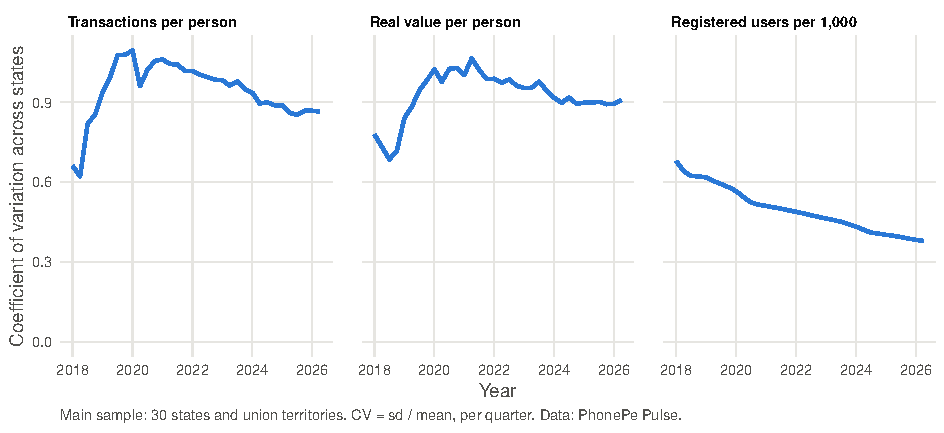
\includegraphics[width=0.96\textwidth,height=0.46\textheight,keepaspectratio]{sigma_convergence.pdf}

{\scriptsize $\sigma$-convergence: coefficient of variation across states, 2018Q1--2026Q2.\par}
\vspace{0.3em}
{\tiny\begin{tblr}[         %% tabularray outer open
]                     %% tabularray outer close
{                     %% tabularray inner open
colspec={Q[]Q[]Q[]},
hline{2}={1-3}{solid, black, 0.05em},
hline{6}={1-3}{solid, black, 0.05em},
hline{1}={1-3}{solid, black, 0.08em},
hline{8}={1-3}{solid, black, 0.08em},
column{2-3}={}{halign=c},
column{1}={}{halign=l},
}                     %% tabularray inner close
& Real value per person & Transactions per person \\
Intercept & 0.3773 & 0.5751 \\
& (0.0788) & (0.0211) \\
ln(initial level) & 0.0174 & -0.0030 \\
& (0.0138) & (0.0128) \\
N & 30 & 30 \\
R2 & 0.054 & 0.002 \\
\end{tblr}

\par}
{\tiny $\beta$-convergence, N = 30, OLS; standard errors in parentheses.\par}
\end{frame}

% ---- 12. NPCI validation
% Source: output/tables/validation_npci.tex; thesis/progress/part2.tex (Validation result)
% Notes: The check covers 2025Q2 to 2026Q2, 5 quarters, 35 ids. State-share correlations are 0.897 to 0.923 (Pearson) and 0.953 to 0.967 (Spearman). Per-capita correlations are 0.615 to 0.742 (Pearson) and 0.455 to 0.605 (Spearman). NPCI unclassified volume is 0.42 to 0.45 of the national total from June 2025.
\begin{frame}{NPCI validation}
\begin{center}
\footnotesize
\resizebox{0.8\textwidth}{!}{\begin{tabular}{lrrrr}
\toprule
 & \multicolumn{2}{c}{Pearson} & \multicolumn{2}{c}{Spearman} \\
\cmidrule(lr){2-3}\cmidrule(lr){4-5}
Quarter & Count share & Value share & Count share & Value share \\
\midrule
2025Q2 & 0.923 & 0.923 & 0.967 & 0.961 \\
2025Q3 & 0.905 & 0.898 & 0.958 & 0.959 \\
2025Q4 & 0.897 & 0.897 & 0.954 & 0.955 \\
2026Q1 & 0.901 & 0.897 & 0.953 & 0.956 \\
2026Q2 & 0.901 & 0.897 & 0.956 & 0.954 \\
\bottomrule
\end{tabular}
}
\end{center}
\begin{itemize}
\item 35 ids, 5 quarters (2025Q2 to 2026Q2). % part2.tex
\item State shares: Pearson 0.897 to 0.923; Spearman 0.953 to 0.967. % part2.tex
\item Per-capita levels: Pearson 0.615 to 0.742; Spearman 0.455 to 0.605. % part2.tex
\item NPCI unclassified volume: 0.42 to 0.45 of the national total from June 2025. % part2.tex
\end{itemize}
\end{frame}

% ---- 13. BTP-II plan
% Source: spec Section 6 (After BTP-I); thesis/btp1/chapters/ch6_plan.tex
% Notes: BTP-II runs December to April. I collect the FI data, build the indices, run Steps 1 to 3, and write the thesis. The paper follows the BTP-II results.
\begin{frame}{Plan for BTP-II}
\begin{itemize}
\item December to April. % spec
\item FI data (RBI BSR, PMJDY, TRAI, NSDP) and quarterly and annual FI indices (PCA; Sarma index as robustness). % ch6_plan.tex
\item Steps 1 to 3: series properties; RQ1, RQ3, RQ4, RQ2; robustness. % ch6_plan.tex
\item Thesis; paper (\texttt{elsarticle}) after the BTP-II results. % spec
\item District-panel extension checked after BTP-I. % spec
\item Blocking items: supervisor acceptance of the PhonePe proxy; department BTP rules. % spec Section 7
\end{itemize}
\end{frame}

% ---- 14. References
% Notes: Sources used in these slides.
\nocite{ncp2020}
\begin{frame}[allowframebreaks]{References}
\tiny
\bibliographystyle{plainnat}
\bibliography{../../references/refs}
\end{frame}

\end{document}
